\newcommand{\editiontag}{ChatGPT edition}
\newcommand{\boundary}{\textbf{Learner boundary:} isolated battery power only,
12 V DC maximum. No outlets, mains leads, opened appliances, large battery
packs, charged power capacitors, ignition coils, sparks, or exposed high
voltage. An adult facilitator is not thereby an electrically qualified person.}
\newenvironment{recordbox}{\begin{teloscard}{Evidence record}\small
\begin{tabularx}{\linewidth}{@{}p{.19\linewidth}L@{}}
Prediction & \rule{.95\linewidth}{.3pt}\\[1.1em]
One change & \rule{.95\linewidth}{.3pt}\\[1.1em]
Observation & \rule{.95\linewidth}{.3pt}\\[1.1em]
Claim + because & \rule{.95\linewidth}{.3pt}
\end{tabularx}}{\end{teloscard}}
\newcommand{\sourcefoot}{\par\smallskip{\footnotesize Physics and safety basis:
NIST SI/CODATA; OSHA 29 CFR 1910.333 and OSHA 3075; DOE Electrical Science
handbooks; HyperPhysics (Georgia State University); University of Colorado
PhET teacher resources. Full citations and scope notes are recorded in the
provider-neutral electricity research library.}}
\newcommand{\rolecard}{\begin{telospanel}{Stop line and roles}\boundary\par
\smallskip The learner predicts, assembles only the pictured battery circuit,
and records. The adult inspects parts, controls power, and stops heat, odor,
damage, pain, or unexpected behavior. Work outside this boundary belongs only
to a person qualified for that work.\end{telospanel}}
\newcommand{\circuitdiagram}{\begin{center}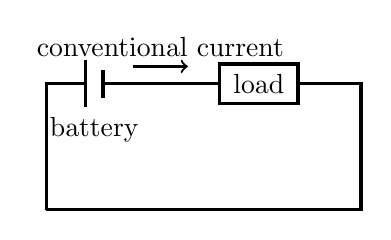
\begin{tikzpicture}[x=1cm,y=1cm]
\draw[very thick] (0,0)--(0,1.6)--(.5,1.6);
\draw[very thick] (.5,1.3)--(.5,1.9); \draw[very thick] (.72,1.42)--(.72,1.78);
\node[below] at (.61,1.3){battery};
\draw[very thick] (.72,1.6)--(2.2,1.6);
\draw[very thick] (2.2,1.35) rectangle (3.2,1.85);
\node at (2.7,1.6){load};
\draw[very thick] (3.2,1.6)--(4,1.6)--(4,0)--(0,0);
\draw[->,thick] (1.1,1.82)--(1.8,1.82) node[midway,above]{conventional current};
\end{tikzpicture}\end{center}}
\newcommand{\fielddiagram}{\begin{center}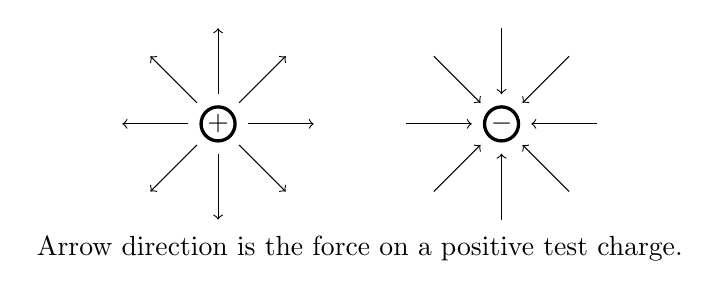
\begin{tikzpicture}[scale=.9]
\draw[very thick] (0,0) circle (.24); \node at (0,0){$+$};
\foreach \a in {0,45,...,315}{\draw[->] ({.42*cos(\a)},{.42*sin(\a)})--({1.35*cos(\a)},{1.35*sin(\a)});}
\draw[very thick] (4,0) circle (.24); \node at (4,0){$-$};
\foreach \a in {0,45,...,315}{\draw[<-] ({4+.42*cos(\a)},{.42*sin(\a)})--({4+1.35*cos(\a)},{1.35*sin(\a)});}
\node[below] at (2,-1.45){Arrow direction is the force on a positive test charge.};
\end{tikzpicture}\end{center}}
\newcommand{\coildiagram}{\begin{center}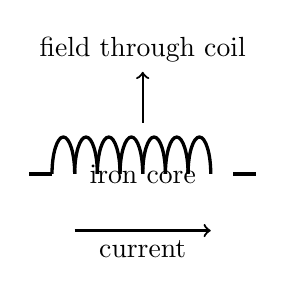
\begin{tikzpicture}[x=.72cm,y=.72cm]
\draw[very thick] (-2,0)--(-1.6,0);
\foreach \x in {-1.6,-1.2,...,1.2}{\draw[very thick] (\x,0) arc (180:0:.2 and .65);}
\draw[very thick] (1.6,0)--(2,0);
\draw[->,thick] (-1.2,-1)--(1.2,-1) node[midway,below]{current};
\draw[->,thick] (0,.9)--(0,1.8) node[above]{field through coil};
\node at (0,0){iron core};
\end{tikzpicture}\end{center}}
\newcommand{\inductiondiagram}{\begin{center}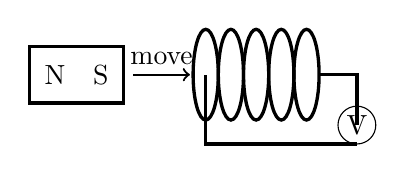
\begin{tikzpicture}[x=.8cm,y=.8cm]
\draw[very thick] (-2,-.45) rectangle (-.5,.45); \node at (-1.25,0){N\quad S};
\draw[->,thick] (-.35,0)--(.55,0) node[midway,above]{move};
\foreach \x in {.8,1.2,...,2.4}{\draw[very thick] (\x,0) ellipse (.2 and .72);}
\draw[very thick] (2.6,0)--(3.2,0)--(3.2,-.8);
\draw (3.2,-.8) circle (.3); \node at (3.2,-.8){V};
\draw[very thick] (3.2,-1.1)--(.8,-1.1)--(.8,0);
\end{tikzpicture}\end{center}}
